%\newpage
\begin{figure}[t]
    \centering
    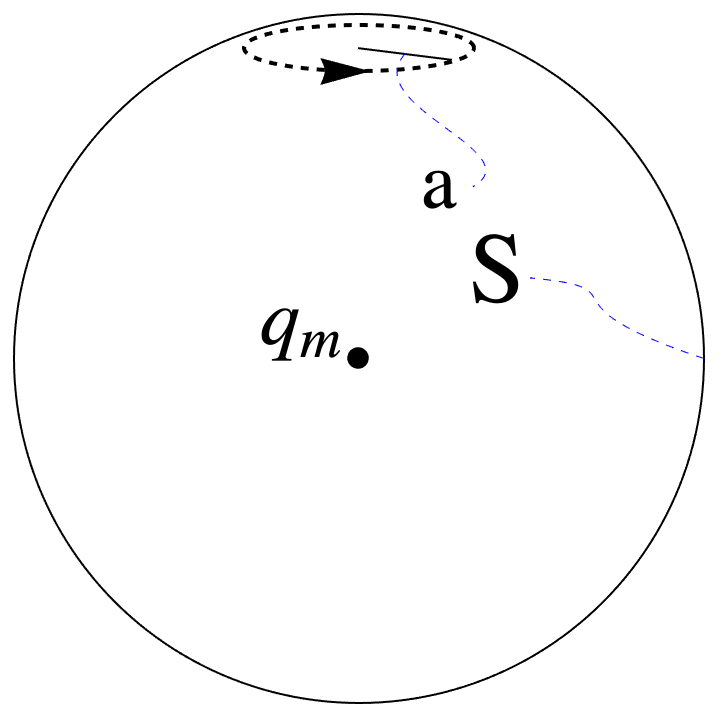
\includegraphics[width=3.5cm, height=3.5cm]{Magnetic Monopole Sketch.png}
    \caption{\textit{Ανοιχτή επιφάνεια $S$. Ο διακεκομμένος κύκλος ακτίνας $a$ είναι σύνορο της $S$}}
    \label{fig:opensurf}
\end{figure}
\section{Συνθήκη Κβάντωσης Dirac}
\noindent Οι συμμετρίες των εξισώσεων \eqref{monem} ωθούν προς την αναζήτηση κάποιου δυναμικού $\Vec{A}$, ικανού να μας δώσει  μέσω της \eqref{curl} ένα κεντρικό μαγνητικό πεδίο. Το μαγνητικό πεδίο $\vec{B}$ πρέπει - όντας ένα μετρήσιμο φυσικό μέγεθος - να είναι καλά ορισμένο παντού στο χώρο, εκτός από τη θέση του σημειακού μονοπόλου ($r = 0$). Η μαγνητική ροή τότε, δίνεται από τον ολοκληρωτικό νόμο Gauss 
\begin{equation}\label{intGauss}
    \int\limits_V \vec{\nabla} \cdot \Vec{B}\, dV = \oint\limits_{\partial V = S} \Vec{B} \cdot d\Vec{s} = 4\pi q_m
\end{equation}

\noindent όπου το επιφανειακό ολοκλήρωμα πραγματοποιείται ως προς την κλειστή επιφάνεια που περιβάλει το μαγνητικό μονόπολο. %- και πρέπει να ισούται με την συνολική μαγνητική ροή διαμέσου %της επιφάνειας. 
%Η 'αδυναμία' του δυναμικού $\vec{A}$ γίνεται εμφανής 
Εάν επιχειρήσουμε να αντικαταστήσουμε την \eqref{curl} στην \eqref{intGauss}, καταλήγοθμε σε μηδενική μαγνητική ροή διαμέσου της επιφάνειας
\begin{equation*}
    \int\limits_V \vec{\nabla} \cdot \left( \vec{\nabla} \times \vec{A} \right) \, dV = 0
\end{equation*}

\subsection{Διανυσματικό δυναμικό με απροσδιοριστίες}
 Για να αποφύγουμε τον μηδενισμό, θα αναθεωρήσουμε το κλειστό επιφανειακό ολοκλήρωμα \eqref{intGauss}. Το ολοκλήρωμα ως προς μια ανοιχτή επιφάνεια $S$ (σχήμα \ref{fig:opensurf}), με βάση το θεώρημα του Stokes, ανάγεται σε επικαμπύλιο και εκτελείται κατά μήκος του κλειστού βρόχου που αποτελεί το σύνορο της ανοιχτής επιφάνειας. Πρέπει να επισημάνουμε ότι αρχικά η διανυσματική συνάρτηση $\vec{A}$ θεωρείται καλά ορισμένη στην $S$:

\begin{equation}\label{lineint}
    \int\limits_{S}  \vec{B} \cdot d\vec{s} = \int\limits_{S}(\vec{\nabla}\times \vec{A} )\cdot d\vec{s} = \oint\limits_{\partial S} \vec{A} \cdot d\vec{\ell}
\end{equation}

Χωρίς βλάβη γενικότητας, επιλέγουμε την $S$ ώστε το σύνορο της να είναι ένας κύκλος με ακτίνα $a$ και άξονα συμμετρίας τον καρτεσιανό άξονα $z$. Το στοιχειώδες μήκος του επικαμπύλιου ολοκληρώματος \eqref{lineint} ισούται με $d\Vec{\ell} = a \,\, d\phi \,\, \hat{\phi}$. Στο όριο όπου η ακτίνα του κύκλου τείνει στο μηδέν, αναμένουμε ότι το επικαμπύλιο ολοκλήρωμα μηδενίζεται, εάν το διανυσματικό δυναμικό είναι παντού καλά ορισμένο, κάτι όμως που οδηγεί σε ασυμφωνία με τη ροή του μονοπόλου:
\begin{equation}\label{limofbound}
    \lim\limits_{a\rightarrow0}\oint\limits_{\partial S} \Vec{A} \cdot \left(  a \,\, d\phi \,\, \hat{\phi} \right) = 0 \quad \ne \oint\limits_{\partial V = S} \Vec{B} \cdot d\Vec{s} 
\end{equation}

\begin{figure}[t]
            \centering
            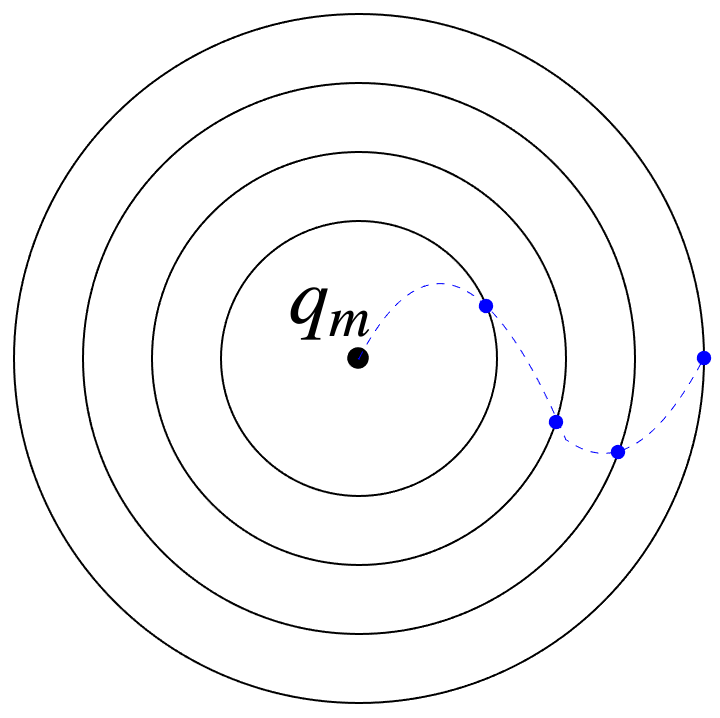
\includegraphics[width=4cm, height=4cm]{Magnetic Monopole String Sketch.png}
            \caption{\textit{Διαδοχικές ομόκεντρες επιφάνειες η κάθε μία από τις οποίες έχει ένα μοναδικό σημείο στο οποίο η συνάρτηση $\vec{A}$ δεν ορίζεται.}}
    \label{fig:diracstr}
\end{figure}
\subsection{Χορδή Dirac}
Για να αναιρέσουμε την ασυμφωνία της \eqref{limofbound}, θεωρούμε λοιπόν ότι το διανυσματικό πεδίο $\vec{A}$ είναι καλά ορισμένο παντού στην $S$, εκτός από ένα σημείο. Έτσι, το επικαμπύλιο ολοκλήρωμα \eqref{limofbound} μπορεί να είναι διάφορο από μηδέν, αλλά πεπερασμένο, ακόμα και στο όριο $a \rightarrow 0$:

\begin{equation*}
            \lim\limits_{a\rightarrow0}\oint\limits_{\partial S} \vec{A} \cdot d\vec{\ell} \ne 0
\end{equation*}
%Η αυθερεσία ως προς τις διαστάσεις της σφαιρικής επιφάνειας S - %που επιβάλλεται όπως περιλαμβάνει την κατανομή φορτίου - %αντικατοπτρίζει την ανεξαρτησία, του θεωρήματος Gauss, από την %επιφάνεια. 
Το θεώρημα Gauss ισχύει για κάθε επιφάνεια που περιβάλει το μαγνητικό μονόπολο, ανεξάρτητα από το σχήμα και το μέγεθος της. Στο σχήμα \ref{fig:diracstr} παρουσιάζονται τέτοιες ομόκεντρες σφαίρες των οποίων τα σημεία απροσδιοριστίας του $\vec{A}$ έχουν τεπιλεγεί και τοποθετηθεί με τέτοιο τρόπο, ώστε για αυθαίρετα μεγάλο αριθμό επιφανειών να σχηματίζουν μια συνεχή καμπύλη. Η καμπύλη αυτή αρχίζει από το σημειακό μονόπολο στο κέντρο και εκτείνεται στο άπειρο. Η καμπύλη ονομάζεται χορδή Dirac. 
%θα επιμείνω σε αυτή την ονομασία για το υπόλοιπο του κειμένου. 
Μια φυσική διάταξη η οποία μπορεί να αναπαραστήσει τη χορδή Dirac, \ref{fig:diracstr}, αποτελεί μια γραμμική κατανομή απειροστά μικρών μαγνητικών διπόλων κατά μήκος ημιευθείας. Η διάταξη αυτή παράγει ένα διανυσματικό δυναμικό με τις ιδιότητες του $\vec{A}$. 
%Αν και στην πραγματικότητα μια ημιάπειρη συνοχή από μαγνητικά %δίπολα δεν είναι υλοποιήσιμη 
Όπως θα δούμε, μετασχηματισμοί βαθμίδας προκαλούν παραμορφώσεις της χορδής Dirac στο χώρο και παράγουν διαφορές φάσεως σε ένα κβαντικό σύστημα.

\subsection{Xορδή Dirac από μαγνητικά δίπολα}
Ένα απειροστό μαγνητικό δίπολο το οποίο αποτελείται από δύο αντίθετα σημειακά μονόπολα $q_m$, $-q_m$, με τη μετατόπιση μεταξύ τους να ισούται με $d\vec{\ell}$, έχει μαγνητική διπολική ροπή
\begin{equation}
    d\vec{m} = q\subscr{m} d\vec{\ell}
\end{equation}
Η συνεισφορά στο διανυσματικό δυναμικό $d\vec{A}$ στη θέση $\vec{x}$ ενός τέτοιου μαγνητικού διπόλου $d\vec{m}$ στη θέση $\vec{x}'$ δίνεται από την έκφραση 
\begin{equation}\label{dipolecontr}
    d\vec{A}(x) \, = \, d\vec{m} \times \frac{(\vec{x}-\pvec{x}')}{|\vec{x}-\pvec{x}'|^3} \, = \, - d\vec{m}\times \vec{\nabla}\left( \frac{1}{|\vec{x}-\pvec{x}'|} \right)
\end{equation}
όπου στη δεύτερη εξίσωση έγινε χρήση της \eqref{apx_1}. 
%\newpage
\begin{figure}[t]
    \centering
    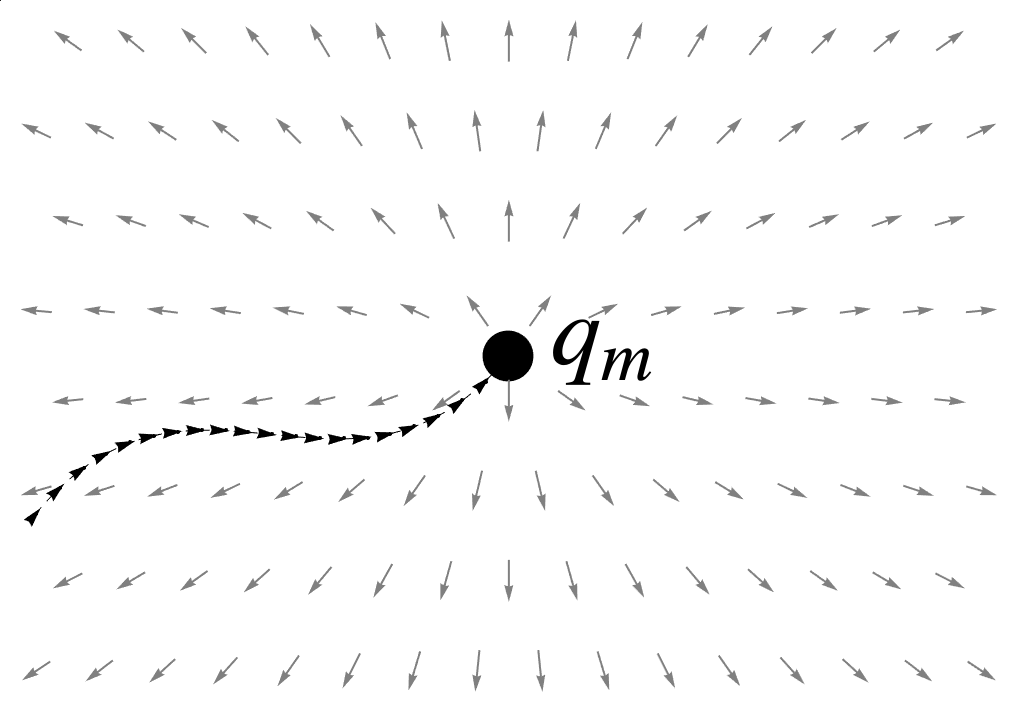
\includegraphics[width=7cm, height=5cm]{monopole field.png}
    \caption{\textit{Μαγνητικά δίπολα (μαύρα βέλη) συνιστούν χορδή Dirac η οποία καταλήγει στο μαγνητικό μονόπολο.}}
    \label{fig:monopfield}
\end{figure}
%Η σύνδεση των πολυάριθμων διπόλων είναι απλά το άθροισμα των %απειροελάχιστα μικρών ροπών που με τη σειρά του γράφεται ως 
Το συνολικό διανυσματικό δυναμικό δίδεται από το επικαμπύλιο ολοκλήρωμα \footnote{$\qquad- d\pvec{\ell}'\times \vec{\nabla}\left(\frac{1}{|\vec{x}-\pvec{x}'|}\right) \, = \, \vec{\nabla}\left(\frac{1}{|\vec{x}-\pvec{x}'|}\right) \times d\pvec{\ell}'\, = \, \vec{\nabla}\times\left(\frac{d\pvec{\ell}'}{|\vec{x}-\pvec{x}'|}\right)$
}
\begin{equation}\label{vectorpot}
    \vec{A}(\vec{x}) \, =  \, -q\subscr{m}\int\limits_L d\pvec{\ell}'\times \vec{\nabla}\left(\frac{1}{|\vec{x}-\pvec{x}'|}\right) \, = \, q\subscr{m}\,\vec{\nabla}\times \int\limits_L \frac{d\pvec{\ell}'}{|\vec{x}-\pvec{x}'|}
\end{equation}
κατά μήκος της χορδής Dirac και ο τελεστής κλίσης δρα στη μεταβλητή $\vec{x}$. Το μαγνητικό πεδίο 
%που αντιστοιχεί στο διανυσματικό δυναμικό της χορδής Dirac, 
%υπολογίζεται ανατρέχοντας πίσω στην εξίσωση 
δίδεται από τη σχέση \eqref{curl}:
%, όπου αντικαθιστούμε την \eqref{vectorpot}. 
\begin{equation}\label{fieldwstr}
\begin{split}
        \Vec{B} &= \vec{\nabla} \times \left( \vec{\nabla} \times \int\limits_L \frac{q\subscr{m}\,d\pvec{\ell}'}{|\vec{x}-\pvec{x}'|}\right)\\
        &= q\subscr{m}\,\vec{\nabla}\int\limits_L \vec{\nabla}\cdot\left(\frac{d\pvec{\ell}'}{|\vec{x}-\pvec{x}'|}\right) - q\subscr{m}\int\limits_L \vec{\nabla}^2\left(\frac{1}{|\vec{x}-\pvec{x}'|}\right)d\pvec{\ell}' \\
        &= \underbrace{q\subscr{m}\frac{\vec{x}-\pvec{x}\subscr{0}}{|\vec{x}-\pvec{x}\subscr{0}|^3}}_{B_{mon}} \, + \, \underbrace{4\pi q\subscr{m} \int\limits_L \delta^3\left(\vec{x}-\pvec{x}'\right)\,d\pvec{\ell}'}_{B_{χορδή}}
\end{split}
\end{equation}
Το άκρο της χορδής βρίσκεται στη θέση $\vec{x}\subscr{0}$. Για την εξαγωγή της δεύτερης ισότητας χρησιμοποιούμε την \eqref{apx_3}. Ο πρώτος όρος του τελικού αποτελέσματος ισούται με το πεδίο του μαγνητικού μονοπόλου. (Οι πράξεις παρουσιάζονται στην \eqref{apx_5}). Ο δεύτερος όρος, βάσει της ταυτότητας \eqref{apx_4}, δείνει το πεδίο της χορδής Dirac, το οποίο δεν προσδιορίζεται. Στο σχήμα \ref{fig:monopfield} αναπαρίσταται γραφικά το συνολικό αποτέλεσμα της \eqref{fieldwstr}. Εχουμε λοιπόν καταλήξει στο ζητούμενο πεδίο του μαγνητικού μονοπόλου, με μια όμως επιπρόσθετη ανεπιθύμητη απροσδιοριστία. Για την εγκυρότητα του πεδίου, επιβάλλεται όπως η απροσδιοριστία αυτή καταστεί μη παρατηρήσιμη. 

%\newpage

\subsection{Μετασχηματισμοί βαθμίδας και χορδή Dirac}
%Σκοπός της παρούσας ενότητας είναι αρχικά η μελέτη της σχέσης %μεταξύ διαμορφώσεων της χορδής Dirac. 
Παρατηρούμε ότι ο πρώτος όρος της \eqref{fieldwstr} είναι ανεξάρτητος του σχήματος της χορδής. Μπορούμε δηλαδή, να παραμορφώσουμε τη χορδή Dirac (αλλάζοντας την καμπύλη $L$), κρατώντας το άκρο της σταθερό, και παίρνουμε το ίδιο πεδίο μαγνητικού μονοπόλου με διαφορετική χορδή.\\

Αντιθέτως, αναμένουμε ότι το διανυσματικό δυναμικό  \eqref{vectorpot} θα μεταβληθεί. Στο πλαίσιο της κβαντικής θεωρίας, η μεταβολή μπορεί να αναπαραχθεί με έναν μετασχηματισμό βαθμίδας \cite{Sakurai:1167961}, ο οποίος μετασχηματίζει τις κυματοσυναρτήσεις
\begin{equation}\label{gtfun}
    \scafun{\Psi}{\vec{x}} \,=\, \scafun[0]{\Psi}{\vec{x}}e^{iq \scafun{\Lambda}{\vec{x}}}
\end{equation}
όπου το $\Lambda$ είναι μια βαθμωτή, μονότιμη και πραγματική συνάρτηση των (x,y,z) και $\Psi_0$ η αρχική κυματοσυνάρτηση. Η κλίση της συνάρτησης $\Lambda$ 
%συσχετίζεται με το αρχικό ($\vecfun[L]{A}{\vec{x}}$) και %μετασχηματισμένο ($\vecfun[L']{A}{\vec{x}}$) 
πρέπει να ισούται με τη μεταβολή του διανυσματικού δυναμικού ως εξής
\begin{equation}\label{gaugetransform}
    \vec{\nabla} \Lambda \,=\, \vecfun[L']{A}{\vec{x}} - \vecfun[L]{A}{\vec{x}}
\end{equation}
Στην περίπτωση της χορδής Dirac όμως, η μεταβολή στο δεξιό μέλος της \eqref{gaugetransform}, αν και μονότιμη συνάρτηση, δεν μπορεί να γραφτεί άμεσα ως η κλίση μιας βαθμωτής συνάρτησης $\Lambda$ εξαιτίας ενός επιπρόσθετου όρου. Στο επόμενο κεφάλαιο θα αποδείξουμε τη συνθήκη κβάντωσης 
%συνθήκη που αποδυκνύει περίτρανα 
του Dirac \cite{Dirac:1931kp}, η οποία καθιστά τις μεταβολές που προκύπτουν, λόγω των παραμορφώσεων της χορδής, μη 
παρατηρήσιμες.\\

Ας θεωρήσουμε λοιπόν δύο χορδές, τις $L$ και $L'$, όπως φαίνεται στο σχήμα \ref{fig:twostrconf}. Επειδή το διανυσματικό δυναμικό ενός μαγνητικού διπόλου
%\footnote{Στο όριο όπου η θέση του διπόλου, $\vec{x}'$ είναι %αρκετά μακριά από τη θέση εξέτασης δυναμικού, $\vec{x}$, έχουμε %\\
%\indent $|d\vec{A}(x)| \, \sim \, %\lim\limits\subscr{|\Vec{x}-\Vec{x}'|\rightarrow %\infty}\frac{1}{|\Vec{x}-\Vec{x}'|^2} \sim 0$ } %\eqref{dipolecontr}, 
φθίνει πολύ γρήγορα (με το τετράγωνο της απόστασης από τη θέση του διπόλου)
μπορούμε, χωρίς βλάβη γενικότητας, να ενώσουμε τις δύο χορδές στο άπειρο. \\

\begin{figure}[t]
    \centering
    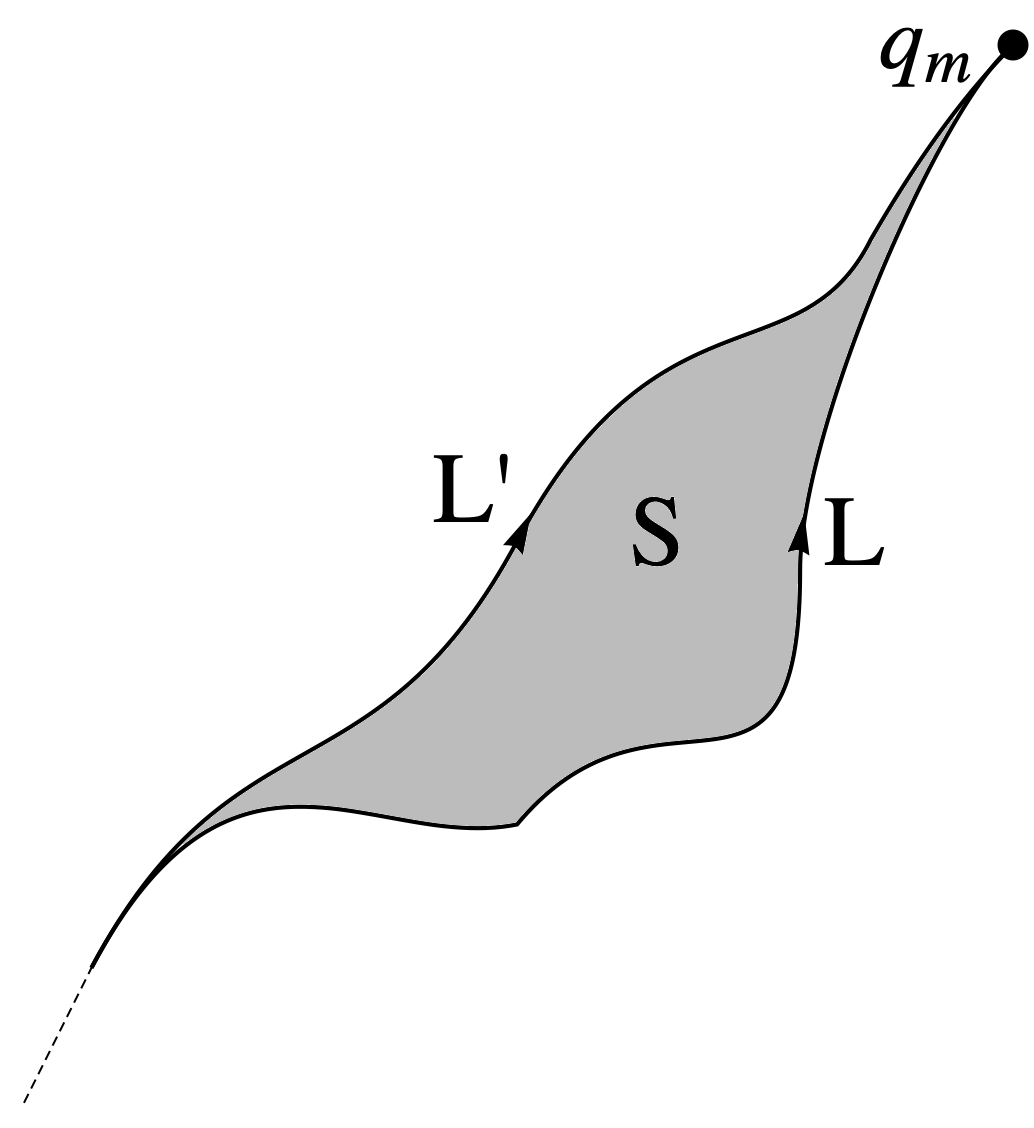
\includegraphics[width=4.5cm, height=4.5cm]{diracstrings}
    \caption{\textit{Δύο ημιάπειρες χορδές Dirac καταλήγουν στο ίδιο σημείο (μαγνητικό μονόπολο). Μακριά από το σημείο όπου απορρέει το μονοπολικό πεδίο, θεωρούμε ότι οι χορδές αλληλοεπικαλύπτονται.}}
    \label{fig:twostrconf}
\end{figure}
%\newpage

Όπως έχουμε ήδη αναφέρει, κάθε χορδή παράγει ένα συγκεκριμένο δυναμικό. Έτσι, για τις δύο χορδές $L$, $L'$ παίρνουμε τα δυναμικά $\vec{A}\subscr{L}$ και $\vec{A}\subscr{L'}$. Η κλειστή διαδρομή $C$, που σχηματίζουν οι δύο χορδές, καθορίζει τη διαφορά των δυναμικών ως εξής
\begin{equation}\label{vecpotdif1}
    \vecfun[L']{A}{\vec{x}} - \vecfun[L]{A}{\vec{x}} \, = \, q\subscr{m}\,\vec{\nabla}\times \left(\int\limits_{L'} \frac{d\pvec{\ell}'}{|\vec{x}-\pvec{x}'|} - \int\limits_L \frac{d\pvec{\ell}'}{|\Vec{x}-\pvec{x}'|} \right) \, = \, q\subscr{m}\,\vec{\nabla}\times \oint\limits_C \frac{d\pvec{\ell}'}{|\Vec{x}-\pvec{x}'|}
\end{equation}

Εφαρμόζουμε τώρα το θεώρημα του Stokes στο κλειστό επικαμπύλιο ολοκλήρωμα της \eqref{vecpotdif1} (παράρτημα \ref{apx22}) και παίρνουμε 
%το επιφανειακό ολοκλήρωμα
\begin{equation}\label{vecpotdif2}
    q\subscr{m}\,\vec{\nabla}\times \oint\limits_C \frac{d\pvec{\ell}'}{|\Vec{x}-\pvec{x}'|}\, =\, q\subscr{m} \, \vec{\nabla}\times\left(\vec{\nabla}\times\int\limits_S \frac{d\pvec{s}'}{|\vec{x}-\pvec{x}'|}\right)
\end{equation}

Με χρήση της ταυτότητας \eqref{apx_3} καταλήγουμε στους ακόλουθους δύο όρους 
\begin{equation}\label{vecpotdif3}
    \vecfun[L']{A}{\vec{x}} - \vecfun[L]{A}{\vec{x}} \,=\, \text{\scalebox{1.5}{$\vec{\nabla}$}} \Bigg(q\subscr{m}\underbrace{\int\limits_S \frac{\pvec{x}'-\vec{x}}{|\vec{x}-\pvec{x}'|^3}\cdot d\pvec{s}'}_{\scafun{\Omega}{\vec{x}}}\Bigg) \,\,\,+\,\,\, 4\pi q\subscr{m} \,\int\limits_S \scafun[][3]{\delta}{\vec{x}-\pvec{x}'} \, d\pvec{s}'
\end{equation}

όπου ο πρώτος όρος είναι η στερεά γωνία που σχηματίζει η επιφάνεια $S$ ως προς το σημείο $\vec{x}$. Ο δεύτερος όρος προκύπτει από την ταυτότητα \eqref{apx_4}. Η διαφορά δυναμικού \eqref{vecpotdif3} εξαρτάται από τη στερεά γωνία της επιφάνειας $S$ μεταξύ των χορδών και ενός απροσδιόριστου όρου - ο οποίος θα αποδειχθεί μη παρατηρήσιμος. \\

\subsection{Συνθήκη κβάντωσης Dirac}

Στο παράδειγμα του παραρτήματος \ref{apx23} γίνεται εφαρμογή των πιο πάνω αποτελεσμάτων και αποδεικνύεται ότι η \eqref{vecpotdif3} μπορεί να ταυτιστεί με ένα μετασχηματισμό βαθμίδας. Συνοπτικά γράφουμε

\begin{equation*}
    L\rightarrow L' \Rightarrow \vecfun[L]{A}{\vec{x}}\rightarrow \vecfun[L']{A}{\vec{x}} \Rightarrow \scafun[0]{\Psi}{\vec{x}} \rightarrow \scafun[0]{\Psi}{\vec{x}}\exp^{iq \scafun{\Lambda}{\vec{x}}}
\end{equation*}
Όταν η χορδή παραμορφώνεται (L$\rightarrow$L') αλλάζει το δυναμικό $\vecfun[L]{A}{\vec{x}}$ και μετασχηματίζονται οι κβαντικές κυματοσυναρτήσεις, βάσει μιας συνάρτησης $\Lambda$ που πρέπει να ικανοποιεί την \eqref{gaugetransform}.\\

Η συνάρτηση $\scafun{\Omega}{\vec{x}}$ στην \eqref{vecpotdif3} %δεν μπορεί να χρησιμοποιηθεί ως η $\Lambda$ λόγω της 
εκδηλώνει ασυνέχεια  διαμέσου της επιφάνειας $S$ του σχήματος \ref{fig:twostrconf}. Πιο συγκεκριμένα, η ασυνέχεια εκδηλώνεται και στη φάση της νέας κυματοσυνάρτησης, ως ακολούθως
\begin{equation}\label{multival}
    \Psi_{L'} = \left\{\begin{array}{cc}
        e^{i\,q\,q_m\Omega_1\Psi_L} & \quad\Vec{x}\rightarrow \vec{x}^{\,-}  \\ \\
        e^{i\,q\,q_m\Omega_2}\Psi_L & \quad\Vec{x}\rightarrow \vec{x}^{\,+}
    \end{array}\right.
\end{equation}
%η οποία συνεπάγεται πλειοτιμία του πλάτους πυκνότητας %πιθανότητας, κάτι που θα την καθιστούσε φυσικά ανυπόστατη. 
Τα σημεία $\vec{x}^{\,-}$ και  $\vec{x}^{\,+}$ απότελούν πλευρικά όρια σημείου της επιφάνειας $S$, καθώς το πλησιάζουμε από τις περιοχές κάτω και πάνω από την επιφάνεια $S$, αντίστοιχα. Οι στερεές γωνίες $\Omega_1 \equiv \scafun{\Omega}{\vec{x}^{\,-}}$ και $\Omega_2 \equiv \scafun{\Omega}{\vec{x}^{\,+}}$ διαφέρουν κατά μια πλήρη στερεά γωνία, ανεξάρτητα της επιφάνειας, δηλ.
\begin{equation*}
    \Omega_1 \,=\, \Omega_2 + 4\pi
\end{equation*} 

%\newpage
Για να είναι λοιπόν η $\Psi_L$ μονότιμη, πρέπει τα δύο πλευρικά όρια \eqref{multival} να ισούνται. Επομένως η ακόλουθη φάση πρέπει να ισούται με τη μονάδα \cite{Dirac:1931kp}
\begin{equation}
    e^{\frac{4\pi\,iq\,q\subscr{m}}{\hbar\,c}} = 1 \quad \Rightarrow \quad \frac{4\pi\,q\,q\subscr{m}}{\hbar\,c} = 2\pi\,n, \quad n=1,2,\dots
\end{equation}

όπου, $q$ το ηλεκτρικό φορτίο του σωματιδίου που περιγράφεται από την κυματοσυνάρτηση. Εάν αντικαταστήσουμε με το στοιχειώδες κβάντο ηλεκτρικού φορτίου, προκύπτει το στοιχειώδες κβάντο μαγνητικού φορτίου: 
\begin{equation}\label{quantum magnetic charge}
    q\subscr{m} \,=\, \frac{\hbar\,c}{2\,e}\qquad (e>0)
\end{equation}